\documentclass[twoside]{book}

% Packages required by doxygen
\usepackage{calc}
\usepackage{doxygen}
\usepackage{graphicx}
\usepackage[utf8]{inputenc}
\usepackage{makeidx}
\usepackage{multicol}
\usepackage{multirow}
\usepackage{fixltx2e}
\PassOptionsToPackage{warn}{textcomp}
\usepackage{textcomp}
\usepackage[nointegrals]{wasysym}
\usepackage[table]{xcolor}

% Font selection
\usepackage[T1]{fontenc}
\usepackage{mathptmx}
\usepackage[scaled=.90]{helvet}
\usepackage{courier}
\usepackage{amssymb}
\usepackage{sectsty}
\renewcommand{\familydefault}{\sfdefault}
\allsectionsfont{%
  \fontseries{bc}\selectfont%
  \color{darkgray}%
}
\renewcommand{\DoxyLabelFont}{%
  \fontseries{bc}\selectfont%
  \color{darkgray}%
}
\newcommand{\+}{\discretionary{\mbox{\scriptsize$\hookleftarrow$}}{}{}}

% Page & text layout
\usepackage{geometry}
\geometry{%
  a4paper,%
  top=2.5cm,%
  bottom=2.5cm,%
  left=2.5cm,%
  right=2.5cm%
}
\tolerance=750
\hfuzz=15pt
\hbadness=750
\setlength{\emergencystretch}{15pt}
\setlength{\parindent}{0cm}
\setlength{\parskip}{0.2cm}
\makeatletter
\renewcommand{\paragraph}{%
  \@startsection{paragraph}{4}{0ex}{-1.0ex}{1.0ex}{%
    \normalfont\normalsize\bfseries\SS@parafont%
  }%
}
\renewcommand{\subparagraph}{%
  \@startsection{subparagraph}{5}{0ex}{-1.0ex}{1.0ex}{%
    \normalfont\normalsize\bfseries\SS@subparafont%
  }%
}
\makeatother

% Headers & footers
\usepackage{fancyhdr}
\pagestyle{fancyplain}
\fancyhead[LE]{\fancyplain{}{\bfseries\thepage}}
\fancyhead[CE]{\fancyplain{}{}}
\fancyhead[RE]{\fancyplain{}{\bfseries\leftmark}}
\fancyhead[LO]{\fancyplain{}{\bfseries\rightmark}}
\fancyhead[CO]{\fancyplain{}{}}
\fancyhead[RO]{\fancyplain{}{\bfseries\thepage}}
\fancyfoot[LE]{\fancyplain{}{}}
\fancyfoot[CE]{\fancyplain{}{}}
\fancyfoot[RE]{\fancyplain{}{\bfseries\scriptsize Generated on Fri Jul 4 2014 12\+:58\+:52 for A\+C\+H\+Clerk by Doxygen }}
\fancyfoot[LO]{\fancyplain{}{\bfseries\scriptsize Generated on Fri Jul 4 2014 12\+:58\+:52 for A\+C\+H\+Clerk by Doxygen }}
\fancyfoot[CO]{\fancyplain{}{}}
\fancyfoot[RO]{\fancyplain{}{}}
\renewcommand{\footrulewidth}{0.4pt}
\renewcommand{\chaptermark}[1]{%
  \markboth{#1}{}%
}
\renewcommand{\sectionmark}[1]{%
  \markright{\thesection\ #1}%
}

% Indices & bibliography
\usepackage{natbib}
\usepackage[titles]{tocloft}
\setcounter{tocdepth}{3}
\setcounter{secnumdepth}{5}
\makeindex

% Hyperlinks (required, but should be loaded last)
\usepackage{ifpdf}
\ifpdf
  \usepackage[pdftex,pagebackref=true]{hyperref}
\else
  \usepackage[ps2pdf,pagebackref=true]{hyperref}
\fi
\hypersetup{%
  colorlinks=true,%
  linkcolor=blue,%
  citecolor=blue,%
  unicode%
}

% Custom commands
\newcommand{\clearemptydoublepage}{%
  \newpage{\pagestyle{empty}\cleardoublepage}%
}


%===== C O N T E N T S =====

\begin{document}

% Titlepage & ToC
\hypersetup{pageanchor=false,
             bookmarks=true,
             bookmarksnumbered=true,
             pdfencoding=unicode
            }
\pagenumbering{roman}
\begin{titlepage}
\vspace*{7cm}
\begin{center}%
{\Large A\+C\+H\+Clerk \\[1ex]\large 1.\+0 }\\
\vspace*{1cm}
{\large Generated by Doxygen 1.8.7}\\
\vspace*{0.5cm}
{\small Fri Jul 4 2014 12:58:52}\\
\end{center}
\end{titlepage}
\clearemptydoublepage
\tableofcontents
\clearemptydoublepage
\pagenumbering{arabic}
\hypersetup{pageanchor=true}

%--- Begin generated contents ---
\chapter{Namespace Index}
\section{Packages}
Here are the packages with brief descriptions (if available)\+:\begin{DoxyCompactList}
\item\contentsline{section}{\hyperlink{namespace_a_c_h_clerk}{A\+C\+H\+Clerk} }{\pageref{namespace_a_c_h_clerk}}{}
\item\contentsline{section}{\hyperlink{namespace_a_c_h_clerk_1_1_properties}{A\+C\+H\+Clerk.\+Properties} }{\pageref{namespace_a_c_h_clerk_1_1_properties}}{}
\end{DoxyCompactList}

\chapter{Hierarchical Index}
\section{Class Hierarchy}
This inheritance list is sorted roughly, but not completely, alphabetically\+:\begin{DoxyCompactList}
\item \contentsline{section}{A\+C\+H\+Clerk.\+Clerk}{\pageref{class_a_c_h_clerk_1_1_clerk}}{}
\item Form\begin{DoxyCompactList}
\item \contentsline{section}{A\+C\+H\+Clerk.\+Clerk\+Form}{\pageref{class_a_c_h_clerk_1_1_clerk_form}}{}
\item \contentsline{section}{A\+C\+H\+Clerk.\+dlg\+Save\+Folder\+Diag}{\pageref{class_a_c_h_clerk_1_1dlg_save_folder_diag}}{}
\item \contentsline{section}{A\+C\+H\+Clerk.\+Preview\+Pane\+Form}{\pageref{class_a_c_h_clerk_1_1_preview_pane_form}}{}
\end{DoxyCompactList}
\item \contentsline{section}{A\+C\+H\+Clerk.\+Packet\+Entry}{\pageref{class_a_c_h_clerk_1_1_packet_entry}}{}
\end{DoxyCompactList}

\chapter{Class Index}
\section{Class List}
Here are the classes, structs, unions and interfaces with brief descriptions\+:\begin{DoxyCompactList}
\item\contentsline{section}{\hyperlink{class_a_c_h_clerk_1_1_clerk}{A\+C\+H\+Clerk.\+Clerk} \\*Public class Clerk.\+cs. Part of the \hyperlink{namespace_a_c_h_clerk}{A\+C\+H\+Clerk} namespace, which represents a program capbable delivering an easy way for employees of the bank to provide A\+C\+H transition packets to customers }{\pageref{class_a_c_h_clerk_1_1_clerk}}{}
\item\contentsline{section}{\hyperlink{class_a_c_h_clerk_1_1_clerk_form}{A\+C\+H\+Clerk.\+Clerk\+Form} }{\pageref{class_a_c_h_clerk_1_1_clerk_form}}{}
\item\contentsline{section}{\hyperlink{class_a_c_h_clerk_1_1dlg_save_folder_diag}{A\+C\+H\+Clerk.\+dlg\+Save\+Folder\+Diag} }{\pageref{class_a_c_h_clerk_1_1dlg_save_folder_diag}}{}
\item\contentsline{section}{\hyperlink{class_a_c_h_clerk_1_1_packet_entry}{A\+C\+H\+Clerk.\+Packet\+Entry} \\*Public class Packet\+Entry.\+cs. Part of the \hyperlink{namespace_a_c_h_clerk}{A\+C\+H\+Clerk} namespace, which represents a program capbable delivering an easy way for employees of the bank to provide A\+C\+H transition packets to customers }{\pageref{class_a_c_h_clerk_1_1_packet_entry}}{}
\item\contentsline{section}{\hyperlink{class_a_c_h_clerk_1_1_preview_pane_form}{A\+C\+H\+Clerk.\+Preview\+Pane\+Form} }{\pageref{class_a_c_h_clerk_1_1_preview_pane_form}}{}
\end{DoxyCompactList}

\chapter{Namespace Documentation}
\hypertarget{namespace_a_c_h_clerk}{\section{Package A\+C\+H\+Clerk}
\label{namespace_a_c_h_clerk}\index{A\+C\+H\+Clerk@{A\+C\+H\+Clerk}}
}
\subsection*{Namespaces}
\begin{DoxyCompactItemize}
\item 
package \hyperlink{namespace_a_c_h_clerk_1_1_properties}{Properties}
\end{DoxyCompactItemize}
\subsection*{Classes}
\begin{DoxyCompactItemize}
\item 
class \hyperlink{class_a_c_h_clerk_1_1_clerk}{Clerk}
\begin{DoxyCompactList}\small\item\em Public class Clerk.\+cs. Part of the \hyperlink{namespace_a_c_h_clerk}{A\+C\+H\+Clerk} namespace, which represents a program capbable delivering an easy way for employees of the bank to provide A\+C\+H transition packets to customers. \end{DoxyCompactList}\item 
class \hyperlink{class_a_c_h_clerk_1_1_clerk_form}{Clerk\+Form}
\item 
class \hyperlink{class_a_c_h_clerk_1_1dlg_save_folder_diag}{dlg\+Save\+Folder\+Diag}
\item 
class \hyperlink{class_a_c_h_clerk_1_1_packet_entry}{Packet\+Entry}
\begin{DoxyCompactList}\small\item\em Public class Packet\+Entry.\+cs. Part of the \hyperlink{namespace_a_c_h_clerk}{A\+C\+H\+Clerk} namespace, which represents a program capbable delivering an easy way for employees of the bank to provide A\+C\+H transition packets to customers. \end{DoxyCompactList}\item 
class \hyperlink{class_a_c_h_clerk_1_1_preview_pane_form}{Preview\+Pane\+Form}
\item 
class {\bfseries Program}
\end{DoxyCompactItemize}

\hypertarget{namespace_a_c_h_clerk_1_1_properties}{\section{Package A\+C\+H\+Clerk.\+Properties}
\label{namespace_a_c_h_clerk_1_1_properties}\index{A\+C\+H\+Clerk.\+Properties@{A\+C\+H\+Clerk.\+Properties}}
}
\subsection*{Classes}
\begin{DoxyCompactItemize}
\item 
class {\bfseries Resources}
\begin{DoxyCompactList}\small\item\em A strongly-\/typed resource class, for looking up localized strings, etc. \end{DoxyCompactList}\item 
class {\bfseries Settings}
\end{DoxyCompactItemize}

\chapter{Class Documentation}
\hypertarget{class_a_c_h_clerk_1_1_clerk}{\section{A\+C\+H\+Clerk.\+Clerk Class Reference}
\label{class_a_c_h_clerk_1_1_clerk}\index{A\+C\+H\+Clerk.\+Clerk@{A\+C\+H\+Clerk.\+Clerk}}
}


Public class Clerk.\+cs. Part of the \hyperlink{namespace_a_c_h_clerk}{A\+C\+H\+Clerk} namespace, which represents a program capbable delivering an easy way for employees of the bank to provide A\+C\+H transition packets to customers.  


\subsection*{Public Member Functions}
\begin{DoxyCompactItemize}
\item 
\hyperlink{class_a_c_h_clerk_1_1_clerk_ac06ec127e87e71de32d5b9290a6e3a81}{Clerk} (String load\+Path)
\begin{DoxyCompactList}\small\item\em Default, public constructor. Sets the parent directory, and allocates memory for the class' collections. \end{DoxyCompactList}\item 
void \hyperlink{class_a_c_h_clerk_1_1_clerk_a8448ab55cbb9a45181a8edb101fa9e95}{Load\+Native\+Change\+Forms} (String path, Boolean Set\+New\+Parent\+Directory)
\begin{DoxyCompactList}\small\item\em Loads the native Change forms. They are all P\+D\+F documents that contain information on switching A\+C\+H transfers between financial institutions. \end{DoxyCompactList}\end{DoxyCompactItemize}
\subsection*{Properties}
\begin{DoxyCompactItemize}
\item 
List$<$ \hyperlink{class_a_c_h_clerk_1_1_packet_entry}{Packet\+Entry} $>$ \hyperlink{class_a_c_h_clerk_1_1_clerk_a6008f6df10bc7cfeef39781e346138b9}{Selected\+Entries}\hspace{0.3cm}{\ttfamily  \mbox{[}get\mbox{]}}
\begin{DoxyCompactList}\small\item\em Returns the selected ach packet entires as an array. This will make it easier to iterate through and compile the final document. \end{DoxyCompactList}\item 
List$<$ \hyperlink{class_a_c_h_clerk_1_1_packet_entry}{Packet\+Entry} $>$ \hyperlink{class_a_c_h_clerk_1_1_clerk_afbfeb34af163cd64ec151b344953d79f}{Native\+Change\+Forms}\hspace{0.3cm}{\ttfamily  \mbox{[}get, set\mbox{]}}
\begin{DoxyCompactList}\small\item\em Returns the native change forms as an array. In case you need to iterate the raw P\+D\+F documents. \end{DoxyCompactList}\item 
int \hyperlink{class_a_c_h_clerk_1_1_clerk_a1c410f7a2fb912b3e62873b5da40323a}{Native\+Forms\+Count}\hspace{0.3cm}{\ttfamily  \mbox{[}get\mbox{]}}
\begin{DoxyCompactList}\small\item\em Number of elements in the native change forms collection. \end{DoxyCompactList}\item 
int \hyperlink{class_a_c_h_clerk_1_1_clerk_a030ee3e580ed999b00e4fd4f4988a5a6}{Selected\+Count}\hspace{0.3cm}{\ttfamily  \mbox{[}get\mbox{]}}
\begin{DoxyCompactList}\small\item\em Number of elements in the selected change forms collection. \end{DoxyCompactList}\item 
String \hyperlink{class_a_c_h_clerk_1_1_clerk_ac896f8970b723c849fb728bbc4fbdefd}{Parent\+Directory}\hspace{0.3cm}{\ttfamily  \mbox{[}get, set\mbox{]}}
\begin{DoxyCompactList}\small\item\em Get or set the parent directory of the clerk file system. \end{DoxyCompactList}\item 
String \hyperlink{class_a_c_h_clerk_1_1_clerk_a1a2f218890be1feeb47819743528531b}{Pre\+Config}\hspace{0.3cm}{\ttfamily  \mbox{[}get, set\mbox{]}}
\begin{DoxyCompactList}\small\item\em Gets the preconfig name. \end{DoxyCompactList}\end{DoxyCompactItemize}


\subsection{Detailed Description}
Public class Clerk.\+cs. Part of the \hyperlink{namespace_a_c_h_clerk}{A\+C\+H\+Clerk} namespace, which represents a program capbable delivering an easy way for employees of the bank to provide A\+C\+H transition packets to customers. 

The \hyperlink{class_a_c_h_clerk_1_1_clerk}{Clerk} represents the main brain of the A\+C\+H packet operation. It is what handles all document manipulation, conversion, presentation, etc.

It is realized, as of v1.\+0, by Clerk\+Form.\+cs.

Author\+: Tyler Vanover. Created\+: 2014-\/06-\/26. Version\+: 1.\+0. 

\subsection{Constructor \& Destructor Documentation}
\hypertarget{class_a_c_h_clerk_1_1_clerk_ac06ec127e87e71de32d5b9290a6e3a81}{\index{A\+C\+H\+Clerk\+::\+Clerk@{A\+C\+H\+Clerk\+::\+Clerk}!Clerk@{Clerk}}
\index{Clerk@{Clerk}!A\+C\+H\+Clerk\+::\+Clerk@{A\+C\+H\+Clerk\+::\+Clerk}}
\subsubsection[{Clerk}]{\setlength{\rightskip}{0pt plus 5cm}A\+C\+H\+Clerk.\+Clerk.\+Clerk (
\begin{DoxyParamCaption}
\item[{String}]{load\+Path}
\end{DoxyParamCaption}
)}}\label{class_a_c_h_clerk_1_1_clerk_ac06ec127e87e71de32d5b9290a6e3a81}


Default, public constructor. Sets the parent directory, and allocates memory for the class' collections. 



\subsection{Member Function Documentation}
\hypertarget{class_a_c_h_clerk_1_1_clerk_a8448ab55cbb9a45181a8edb101fa9e95}{\index{A\+C\+H\+Clerk\+::\+Clerk@{A\+C\+H\+Clerk\+::\+Clerk}!Load\+Native\+Change\+Forms@{Load\+Native\+Change\+Forms}}
\index{Load\+Native\+Change\+Forms@{Load\+Native\+Change\+Forms}!A\+C\+H\+Clerk\+::\+Clerk@{A\+C\+H\+Clerk\+::\+Clerk}}
\subsubsection[{Load\+Native\+Change\+Forms}]{\setlength{\rightskip}{0pt plus 5cm}void A\+C\+H\+Clerk.\+Clerk.\+Load\+Native\+Change\+Forms (
\begin{DoxyParamCaption}
\item[{String}]{path, }
\item[{Boolean}]{Set\+New\+Parent\+Directory}
\end{DoxyParamCaption}
)}}\label{class_a_c_h_clerk_1_1_clerk_a8448ab55cbb9a45181a8edb101fa9e95}


Loads the native Change forms. They are all P\+D\+F documents that contain information on switching A\+C\+H transfers between financial institutions. 


\begin{DoxyParams}{Parameters}
{\em path} & Path to load the native forms from.\\
\hline
{\em Set\+New\+Parent\+Directory} & Set \char`\"{}\+True\char`\"{} to overwrite the current Parent\+Directory.\\
\hline
\end{DoxyParams}
\begin{DoxyReturn}{Returns}
Void.
\end{DoxyReturn}


\subsection{Property Documentation}
\hypertarget{class_a_c_h_clerk_1_1_clerk_afbfeb34af163cd64ec151b344953d79f}{\index{A\+C\+H\+Clerk\+::\+Clerk@{A\+C\+H\+Clerk\+::\+Clerk}!Native\+Change\+Forms@{Native\+Change\+Forms}}
\index{Native\+Change\+Forms@{Native\+Change\+Forms}!A\+C\+H\+Clerk\+::\+Clerk@{A\+C\+H\+Clerk\+::\+Clerk}}
\subsubsection[{Native\+Change\+Forms}]{\setlength{\rightskip}{0pt plus 5cm}List$<${\bf Packet\+Entry}$>$ A\+C\+H\+Clerk.\+Clerk.\+Native\+Change\+Forms\hspace{0.3cm}{\ttfamily [get]}, {\ttfamily [set]}}}\label{class_a_c_h_clerk_1_1_clerk_afbfeb34af163cd64ec151b344953d79f}


Returns the native change forms as an array. In case you need to iterate the raw P\+D\+F documents. 

\hypertarget{class_a_c_h_clerk_1_1_clerk_a1c410f7a2fb912b3e62873b5da40323a}{\index{A\+C\+H\+Clerk\+::\+Clerk@{A\+C\+H\+Clerk\+::\+Clerk}!Native\+Forms\+Count@{Native\+Forms\+Count}}
\index{Native\+Forms\+Count@{Native\+Forms\+Count}!A\+C\+H\+Clerk\+::\+Clerk@{A\+C\+H\+Clerk\+::\+Clerk}}
\subsubsection[{Native\+Forms\+Count}]{\setlength{\rightskip}{0pt plus 5cm}int A\+C\+H\+Clerk.\+Clerk.\+Native\+Forms\+Count\hspace{0.3cm}{\ttfamily [get]}}}\label{class_a_c_h_clerk_1_1_clerk_a1c410f7a2fb912b3e62873b5da40323a}


Number of elements in the native change forms collection. 

\hypertarget{class_a_c_h_clerk_1_1_clerk_ac896f8970b723c849fb728bbc4fbdefd}{\index{A\+C\+H\+Clerk\+::\+Clerk@{A\+C\+H\+Clerk\+::\+Clerk}!Parent\+Directory@{Parent\+Directory}}
\index{Parent\+Directory@{Parent\+Directory}!A\+C\+H\+Clerk\+::\+Clerk@{A\+C\+H\+Clerk\+::\+Clerk}}
\subsubsection[{Parent\+Directory}]{\setlength{\rightskip}{0pt plus 5cm}String A\+C\+H\+Clerk.\+Clerk.\+Parent\+Directory\hspace{0.3cm}{\ttfamily [get]}, {\ttfamily [set]}}}\label{class_a_c_h_clerk_1_1_clerk_ac896f8970b723c849fb728bbc4fbdefd}


Get or set the parent directory of the clerk file system. 

\hypertarget{class_a_c_h_clerk_1_1_clerk_a1a2f218890be1feeb47819743528531b}{\index{A\+C\+H\+Clerk\+::\+Clerk@{A\+C\+H\+Clerk\+::\+Clerk}!Pre\+Config@{Pre\+Config}}
\index{Pre\+Config@{Pre\+Config}!A\+C\+H\+Clerk\+::\+Clerk@{A\+C\+H\+Clerk\+::\+Clerk}}
\subsubsection[{Pre\+Config}]{\setlength{\rightskip}{0pt plus 5cm}String A\+C\+H\+Clerk.\+Clerk.\+Pre\+Config\hspace{0.3cm}{\ttfamily [get]}, {\ttfamily [set]}}}\label{class_a_c_h_clerk_1_1_clerk_a1a2f218890be1feeb47819743528531b}


Gets the preconfig name. 

\hypertarget{class_a_c_h_clerk_1_1_clerk_a030ee3e580ed999b00e4fd4f4988a5a6}{\index{A\+C\+H\+Clerk\+::\+Clerk@{A\+C\+H\+Clerk\+::\+Clerk}!Selected\+Count@{Selected\+Count}}
\index{Selected\+Count@{Selected\+Count}!A\+C\+H\+Clerk\+::\+Clerk@{A\+C\+H\+Clerk\+::\+Clerk}}
\subsubsection[{Selected\+Count}]{\setlength{\rightskip}{0pt plus 5cm}int A\+C\+H\+Clerk.\+Clerk.\+Selected\+Count\hspace{0.3cm}{\ttfamily [get]}}}\label{class_a_c_h_clerk_1_1_clerk_a030ee3e580ed999b00e4fd4f4988a5a6}


Number of elements in the selected change forms collection. 

\hypertarget{class_a_c_h_clerk_1_1_clerk_a6008f6df10bc7cfeef39781e346138b9}{\index{A\+C\+H\+Clerk\+::\+Clerk@{A\+C\+H\+Clerk\+::\+Clerk}!Selected\+Entries@{Selected\+Entries}}
\index{Selected\+Entries@{Selected\+Entries}!A\+C\+H\+Clerk\+::\+Clerk@{A\+C\+H\+Clerk\+::\+Clerk}}
\subsubsection[{Selected\+Entries}]{\setlength{\rightskip}{0pt plus 5cm}List$<${\bf Packet\+Entry}$>$ A\+C\+H\+Clerk.\+Clerk.\+Selected\+Entries\hspace{0.3cm}{\ttfamily [get]}}}\label{class_a_c_h_clerk_1_1_clerk_a6008f6df10bc7cfeef39781e346138b9}


Returns the selected ach packet entires as an array. This will make it easier to iterate through and compile the final document. 



The documentation for this class was generated from the following file\+:\begin{DoxyCompactItemize}
\item 
Clerk.\+cs\end{DoxyCompactItemize}

\hypertarget{class_a_c_h_clerk_1_1_clerk_form}{\section{A\+C\+H\+Clerk.\+Clerk\+Form Class Reference}
\label{class_a_c_h_clerk_1_1_clerk_form}\index{A\+C\+H\+Clerk.\+Clerk\+Form@{A\+C\+H\+Clerk.\+Clerk\+Form}}
}
Inheritance diagram for A\+C\+H\+Clerk.\+Clerk\+Form\+:\begin{figure}[H]
\begin{center}
\leavevmode
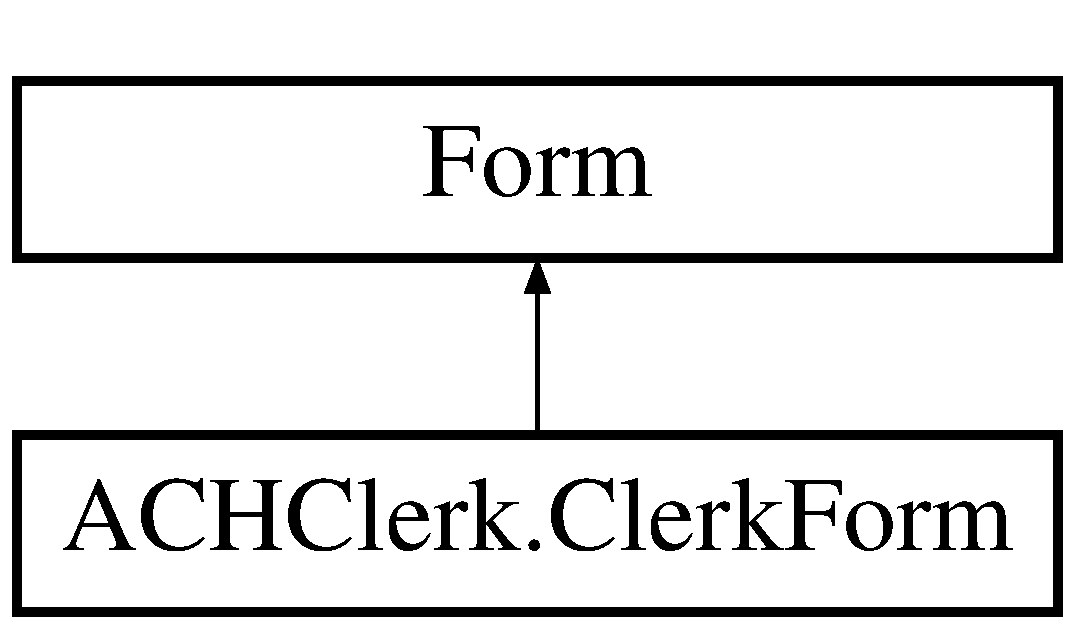
\includegraphics[height=2.000000cm]{class_a_c_h_clerk_1_1_clerk_form}
\end{center}
\end{figure}
\subsection*{Protected Member Functions}
\begin{DoxyCompactItemize}
\item 
override void \hyperlink{class_a_c_h_clerk_1_1_clerk_form_ad06c260cb81e1a91dde602fb741b811f}{Dispose} (bool disposing)
\begin{DoxyCompactList}\small\item\em Clean up any resources being used. \end{DoxyCompactList}\end{DoxyCompactItemize}


\subsection{Member Function Documentation}
\hypertarget{class_a_c_h_clerk_1_1_clerk_form_ad06c260cb81e1a91dde602fb741b811f}{\index{A\+C\+H\+Clerk\+::\+Clerk\+Form@{A\+C\+H\+Clerk\+::\+Clerk\+Form}!Dispose@{Dispose}}
\index{Dispose@{Dispose}!A\+C\+H\+Clerk\+::\+Clerk\+Form@{A\+C\+H\+Clerk\+::\+Clerk\+Form}}
\subsubsection[{Dispose}]{\setlength{\rightskip}{0pt plus 5cm}override void A\+C\+H\+Clerk.\+Clerk\+Form.\+Dispose (
\begin{DoxyParamCaption}
\item[{bool}]{disposing}
\end{DoxyParamCaption}
)\hspace{0.3cm}{\ttfamily [protected]}}}\label{class_a_c_h_clerk_1_1_clerk_form_ad06c260cb81e1a91dde602fb741b811f}


Clean up any resources being used. 


\begin{DoxyParams}{Parameters}
{\em disposing} & true if managed resources should be disposed; otherwise, false.\\
\hline
\end{DoxyParams}


The documentation for this class was generated from the following files\+:\begin{DoxyCompactItemize}
\item 
Clerk\+Form.\+cs\item 
Clerk\+Form.\+Designer.\+cs\end{DoxyCompactItemize}

\hypertarget{class_a_c_h_clerk_1_1dlg_save_folder_diag}{\section{A\+C\+H\+Clerk.\+dlg\+Save\+Folder\+Diag Class Reference}
\label{class_a_c_h_clerk_1_1dlg_save_folder_diag}\index{A\+C\+H\+Clerk.\+dlg\+Save\+Folder\+Diag@{A\+C\+H\+Clerk.\+dlg\+Save\+Folder\+Diag}}
}
Inheritance diagram for A\+C\+H\+Clerk.\+dlg\+Save\+Folder\+Diag\+:\begin{figure}[H]
\begin{center}
\leavevmode
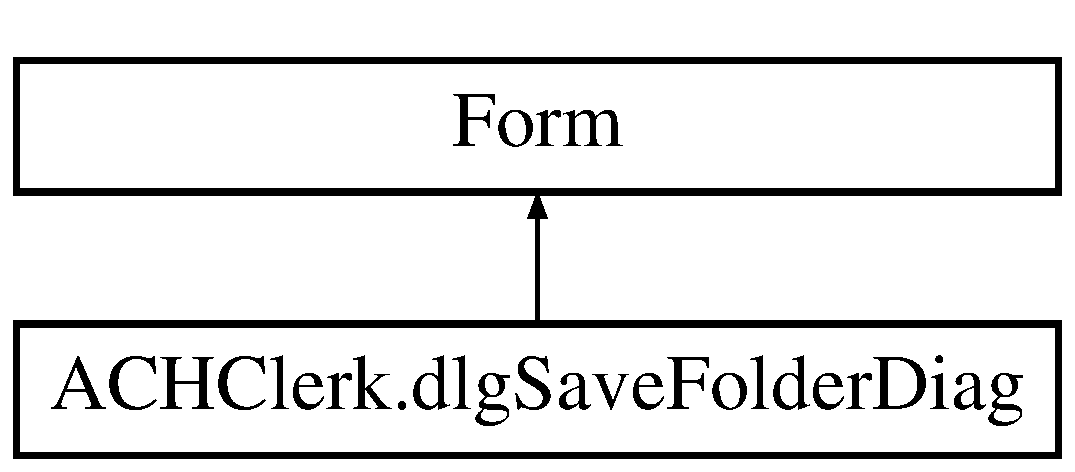
\includegraphics[height=2.000000cm]{class_a_c_h_clerk_1_1dlg_save_folder_diag}
\end{center}
\end{figure}
\subsection*{Public Member Functions}
\begin{DoxyCompactItemize}
\item 
\hyperlink{class_a_c_h_clerk_1_1dlg_save_folder_diag_ab1756da02d4d179151f710f1e36e9edc}{dlg\+Save\+Folder\+Diag} ()
\begin{DoxyCompactList}\small\item\em Public, default constructor. \end{DoxyCompactList}\item 
\hyperlink{class_a_c_h_clerk_1_1dlg_save_folder_diag_a7398a9b24c8813f4ff91d7868f0bf180}{dlg\+Save\+Folder\+Diag} (ref \hyperlink{class_a_c_h_clerk_1_1_clerk}{Clerk} clerk, String path)
\begin{DoxyCompactList}\small\item\em Public, non-\/default constructor. Allows for the clerk to receive information back from the dialog. \end{DoxyCompactList}\end{DoxyCompactItemize}
\subsection*{Protected Member Functions}
\begin{DoxyCompactItemize}
\item 
override void \hyperlink{class_a_c_h_clerk_1_1dlg_save_folder_diag_ad72fba8b0b331fceac2db6c0a016cd50}{Dispose} (bool disposing)
\begin{DoxyCompactList}\small\item\em Clean up any resources being used. \end{DoxyCompactList}\end{DoxyCompactItemize}
\subsection*{Properties}
\begin{DoxyCompactItemize}
\item 
bool \hyperlink{class_a_c_h_clerk_1_1dlg_save_folder_diag_aba57061da5bffd3613ebe82cf81269fc}{Is\+Checked}\hspace{0.3cm}{\ttfamily  \mbox{[}get, set\mbox{]}}
\begin{DoxyCompactList}\small\item\em Gets or privately sets the status of the checkbox button. \end{DoxyCompactList}\end{DoxyCompactItemize}


\subsection{Constructor \& Destructor Documentation}
\hypertarget{class_a_c_h_clerk_1_1dlg_save_folder_diag_ab1756da02d4d179151f710f1e36e9edc}{\index{A\+C\+H\+Clerk\+::dlg\+Save\+Folder\+Diag@{A\+C\+H\+Clerk\+::dlg\+Save\+Folder\+Diag}!dlg\+Save\+Folder\+Diag@{dlg\+Save\+Folder\+Diag}}
\index{dlg\+Save\+Folder\+Diag@{dlg\+Save\+Folder\+Diag}!A\+C\+H\+Clerk\+::dlg\+Save\+Folder\+Diag@{A\+C\+H\+Clerk\+::dlg\+Save\+Folder\+Diag}}
\subsubsection[{dlg\+Save\+Folder\+Diag}]{\setlength{\rightskip}{0pt plus 5cm}A\+C\+H\+Clerk.\+dlg\+Save\+Folder\+Diag.\+dlg\+Save\+Folder\+Diag (
\begin{DoxyParamCaption}
{}
\end{DoxyParamCaption}
)}}\label{class_a_c_h_clerk_1_1dlg_save_folder_diag_ab1756da02d4d179151f710f1e36e9edc}


Public, default constructor. 

\hypertarget{class_a_c_h_clerk_1_1dlg_save_folder_diag_a7398a9b24c8813f4ff91d7868f0bf180}{\index{A\+C\+H\+Clerk\+::dlg\+Save\+Folder\+Diag@{A\+C\+H\+Clerk\+::dlg\+Save\+Folder\+Diag}!dlg\+Save\+Folder\+Diag@{dlg\+Save\+Folder\+Diag}}
\index{dlg\+Save\+Folder\+Diag@{dlg\+Save\+Folder\+Diag}!A\+C\+H\+Clerk\+::dlg\+Save\+Folder\+Diag@{A\+C\+H\+Clerk\+::dlg\+Save\+Folder\+Diag}}
\subsubsection[{dlg\+Save\+Folder\+Diag}]{\setlength{\rightskip}{0pt plus 5cm}A\+C\+H\+Clerk.\+dlg\+Save\+Folder\+Diag.\+dlg\+Save\+Folder\+Diag (
\begin{DoxyParamCaption}
\item[{ref {\bf Clerk}}]{clerk, }
\item[{String}]{path}
\end{DoxyParamCaption}
)}}\label{class_a_c_h_clerk_1_1dlg_save_folder_diag_a7398a9b24c8813f4ff91d7868f0bf180}


Public, non-\/default constructor. Allows for the clerk to receive information back from the dialog. 


\begin{DoxyParams}{Parameters}
{\em clerk} & \\
\hline
\end{DoxyParams}


\subsection{Member Function Documentation}
\hypertarget{class_a_c_h_clerk_1_1dlg_save_folder_diag_ad72fba8b0b331fceac2db6c0a016cd50}{\index{A\+C\+H\+Clerk\+::dlg\+Save\+Folder\+Diag@{A\+C\+H\+Clerk\+::dlg\+Save\+Folder\+Diag}!Dispose@{Dispose}}
\index{Dispose@{Dispose}!A\+C\+H\+Clerk\+::dlg\+Save\+Folder\+Diag@{A\+C\+H\+Clerk\+::dlg\+Save\+Folder\+Diag}}
\subsubsection[{Dispose}]{\setlength{\rightskip}{0pt plus 5cm}override void A\+C\+H\+Clerk.\+dlg\+Save\+Folder\+Diag.\+Dispose (
\begin{DoxyParamCaption}
\item[{bool}]{disposing}
\end{DoxyParamCaption}
)\hspace{0.3cm}{\ttfamily [protected]}}}\label{class_a_c_h_clerk_1_1dlg_save_folder_diag_ad72fba8b0b331fceac2db6c0a016cd50}


Clean up any resources being used. 


\begin{DoxyParams}{Parameters}
{\em disposing} & true if managed resources should be disposed; otherwise, false.\\
\hline
\end{DoxyParams}


\subsection{Property Documentation}
\hypertarget{class_a_c_h_clerk_1_1dlg_save_folder_diag_aba57061da5bffd3613ebe82cf81269fc}{\index{A\+C\+H\+Clerk\+::dlg\+Save\+Folder\+Diag@{A\+C\+H\+Clerk\+::dlg\+Save\+Folder\+Diag}!Is\+Checked@{Is\+Checked}}
\index{Is\+Checked@{Is\+Checked}!A\+C\+H\+Clerk\+::dlg\+Save\+Folder\+Diag@{A\+C\+H\+Clerk\+::dlg\+Save\+Folder\+Diag}}
\subsubsection[{Is\+Checked}]{\setlength{\rightskip}{0pt plus 5cm}bool A\+C\+H\+Clerk.\+dlg\+Save\+Folder\+Diag.\+Is\+Checked\hspace{0.3cm}{\ttfamily [get]}, {\ttfamily [set]}}}\label{class_a_c_h_clerk_1_1dlg_save_folder_diag_aba57061da5bffd3613ebe82cf81269fc}


Gets or privately sets the status of the checkbox button. 



The documentation for this class was generated from the following files\+:\begin{DoxyCompactItemize}
\item 
Save\+Folder\+Form.\+cs\item 
Save\+Folder\+Form.\+Designer.\+cs\end{DoxyCompactItemize}

\hypertarget{class_a_c_h_clerk_1_1_packet_entry}{\section{A\+C\+H\+Clerk.\+Packet\+Entry Class Reference}
\label{class_a_c_h_clerk_1_1_packet_entry}\index{A\+C\+H\+Clerk.\+Packet\+Entry@{A\+C\+H\+Clerk.\+Packet\+Entry}}
}


Public class Packet\+Entry.\+cs. Part of the \hyperlink{namespace_a_c_h_clerk}{A\+C\+H\+Clerk} namespace, which represents a program capbable delivering an easy way for employees of the bank to provide A\+C\+H transition packets to customers.  


\subsection*{Public Member Functions}
\begin{DoxyCompactItemize}
\item 
\hypertarget{class_a_c_h_clerk_1_1_packet_entry_ac7d87dd3e746dc246c08fb42fd9e733d}{{\bfseries Packet\+Entry} (int packet\+I\+D, Pdf\+Document native, String company, ref List$<$ String $>$ tags, bool is\+Table)}\label{class_a_c_h_clerk_1_1_packet_entry_ac7d87dd3e746dc246c08fb42fd9e733d}

\item 
override String \hyperlink{class_a_c_h_clerk_1_1_packet_entry_a08b5203632609dad4bc69c1251d8f444}{To\+String} ()
\begin{DoxyCompactList}\small\item\em Overrides the To\+String function, returning the \hyperlink{class_a_c_h_clerk_1_1_packet_entry}{Packet\+Entry} as a string. This is very rough, as of now, and will require refinement as the project progresses. \end{DoxyCompactList}\end{DoxyCompactItemize}
\subsection*{Properties}
\begin{DoxyCompactItemize}
\item 
Pdf\+Document \hyperlink{class_a_c_h_clerk_1_1_packet_entry_ab19c84887a206d860b73e2a1ac418459}{Native\+Doc}\hspace{0.3cm}{\ttfamily  \mbox{[}get, set\mbox{]}}
\begin{DoxyCompactList}\small\item\em Assigns or returns the native Pdf\+Document attached to this packet entry. Will allow for rendering of individual packet entries as applied to a list box/combo box on a viewing pane. \end{DoxyCompactList}\item 
int \hyperlink{class_a_c_h_clerk_1_1_packet_entry_a1a2d184afd1ab9b8aaccf0ac9bdb5d62}{Packet\+I\+D}\hspace{0.3cm}{\ttfamily  \mbox{[}get, set\mbox{]}}
\begin{DoxyCompactList}\small\item\em Assigns or returns the packet entry's I\+D number. \end{DoxyCompactList}\item 
String \hyperlink{class_a_c_h_clerk_1_1_packet_entry_adc6526f8427f62955cf5353e7067fff5}{Company}\hspace{0.3cm}{\ttfamily  \mbox{[}get, set\mbox{]}}
\begin{DoxyCompactList}\small\item\em Assigns or returns the packet entry's company. \end{DoxyCompactList}\item 
List$<$ String $>$ \hyperlink{class_a_c_h_clerk_1_1_packet_entry_aa0e26c66a7884c983e91a014b6766f5e}{Tags}\hspace{0.3cm}{\ttfamily  \mbox{[}get, set\mbox{]}}
\begin{DoxyCompactList}\small\item\em Returns an array of the various service tags applied to this packet entry. Will be used for a tree-\/based search. \end{DoxyCompactList}\item 
int \hyperlink{class_a_c_h_clerk_1_1_packet_entry_ae73ddc1eccfe1906754fbf36101e66eb}{Tags\+Count}\hspace{0.3cm}{\ttfamily  \mbox{[}get\mbox{]}}
\begin{DoxyCompactList}\small\item\em Returns the number of tags associated with each P\+D\+F packet. \end{DoxyCompactList}\item 
bool \hyperlink{class_a_c_h_clerk_1_1_packet_entry_a4a1c4084b79b907b6a4f8ef9b91ba042}{Is\+Table}\hspace{0.3cm}{\ttfamily  \mbox{[}get, set\mbox{]}}
\begin{DoxyCompactList}\small\item\em Determines if the packet entry is a table. Will allow for easier manipulation later on when compiling tables. \end{DoxyCompactList}\end{DoxyCompactItemize}


\subsection{Detailed Description}
Public class Packet\+Entry.\+cs. Part of the \hyperlink{namespace_a_c_h_clerk}{A\+C\+H\+Clerk} namespace, which represents a program capbable delivering an easy way for employees of the bank to provide A\+C\+H transition packets to customers. 

A \hyperlink{class_a_c_h_clerk_1_1_packet_entry}{Packet\+Entry} is simply a collection of features regarding a single P\+D\+F document. Each \hyperlink{class_a_c_h_clerk_1_1_packet_entry}{Packet\+Entry} has a unique I\+D, a company name, and a list of tags -- the list of tags will the user to type in a string in the search bar and have a number of documents show as a result.

Author\+: Tyler Vanover. Created\+: 2014-\/06-\/26. Version\+: 1.\+0. 

\subsection{Member Function Documentation}
\hypertarget{class_a_c_h_clerk_1_1_packet_entry_a08b5203632609dad4bc69c1251d8f444}{\index{A\+C\+H\+Clerk\+::\+Packet\+Entry@{A\+C\+H\+Clerk\+::\+Packet\+Entry}!To\+String@{To\+String}}
\index{To\+String@{To\+String}!A\+C\+H\+Clerk\+::\+Packet\+Entry@{A\+C\+H\+Clerk\+::\+Packet\+Entry}}
\subsubsection[{To\+String}]{\setlength{\rightskip}{0pt plus 5cm}override String A\+C\+H\+Clerk.\+Packet\+Entry.\+To\+String (
\begin{DoxyParamCaption}
{}
\end{DoxyParamCaption}
)}}\label{class_a_c_h_clerk_1_1_packet_entry_a08b5203632609dad4bc69c1251d8f444}


Overrides the To\+String function, returning the \hyperlink{class_a_c_h_clerk_1_1_packet_entry}{Packet\+Entry} as a string. This is very rough, as of now, and will require refinement as the project progresses. 

\begin{DoxyReturn}{Returns}

\end{DoxyReturn}


\subsection{Property Documentation}
\hypertarget{class_a_c_h_clerk_1_1_packet_entry_adc6526f8427f62955cf5353e7067fff5}{\index{A\+C\+H\+Clerk\+::\+Packet\+Entry@{A\+C\+H\+Clerk\+::\+Packet\+Entry}!Company@{Company}}
\index{Company@{Company}!A\+C\+H\+Clerk\+::\+Packet\+Entry@{A\+C\+H\+Clerk\+::\+Packet\+Entry}}
\subsubsection[{Company}]{\setlength{\rightskip}{0pt plus 5cm}String A\+C\+H\+Clerk.\+Packet\+Entry.\+Company\hspace{0.3cm}{\ttfamily [get]}, {\ttfamily [set]}}}\label{class_a_c_h_clerk_1_1_packet_entry_adc6526f8427f62955cf5353e7067fff5}


Assigns or returns the packet entry's company. 

\hypertarget{class_a_c_h_clerk_1_1_packet_entry_a4a1c4084b79b907b6a4f8ef9b91ba042}{\index{A\+C\+H\+Clerk\+::\+Packet\+Entry@{A\+C\+H\+Clerk\+::\+Packet\+Entry}!Is\+Table@{Is\+Table}}
\index{Is\+Table@{Is\+Table}!A\+C\+H\+Clerk\+::\+Packet\+Entry@{A\+C\+H\+Clerk\+::\+Packet\+Entry}}
\subsubsection[{Is\+Table}]{\setlength{\rightskip}{0pt plus 5cm}bool A\+C\+H\+Clerk.\+Packet\+Entry.\+Is\+Table\hspace{0.3cm}{\ttfamily [get]}, {\ttfamily [set]}}}\label{class_a_c_h_clerk_1_1_packet_entry_a4a1c4084b79b907b6a4f8ef9b91ba042}


Determines if the packet entry is a table. Will allow for easier manipulation later on when compiling tables. 

\hypertarget{class_a_c_h_clerk_1_1_packet_entry_ab19c84887a206d860b73e2a1ac418459}{\index{A\+C\+H\+Clerk\+::\+Packet\+Entry@{A\+C\+H\+Clerk\+::\+Packet\+Entry}!Native\+Doc@{Native\+Doc}}
\index{Native\+Doc@{Native\+Doc}!A\+C\+H\+Clerk\+::\+Packet\+Entry@{A\+C\+H\+Clerk\+::\+Packet\+Entry}}
\subsubsection[{Native\+Doc}]{\setlength{\rightskip}{0pt plus 5cm}Pdf\+Document A\+C\+H\+Clerk.\+Packet\+Entry.\+Native\+Doc\hspace{0.3cm}{\ttfamily [get]}, {\ttfamily [set]}}}\label{class_a_c_h_clerk_1_1_packet_entry_ab19c84887a206d860b73e2a1ac418459}


Assigns or returns the native Pdf\+Document attached to this packet entry. Will allow for rendering of individual packet entries as applied to a list box/combo box on a viewing pane. 

\hypertarget{class_a_c_h_clerk_1_1_packet_entry_a1a2d184afd1ab9b8aaccf0ac9bdb5d62}{\index{A\+C\+H\+Clerk\+::\+Packet\+Entry@{A\+C\+H\+Clerk\+::\+Packet\+Entry}!Packet\+I\+D@{Packet\+I\+D}}
\index{Packet\+I\+D@{Packet\+I\+D}!A\+C\+H\+Clerk\+::\+Packet\+Entry@{A\+C\+H\+Clerk\+::\+Packet\+Entry}}
\subsubsection[{Packet\+I\+D}]{\setlength{\rightskip}{0pt plus 5cm}int A\+C\+H\+Clerk.\+Packet\+Entry.\+Packet\+I\+D\hspace{0.3cm}{\ttfamily [get]}, {\ttfamily [set]}}}\label{class_a_c_h_clerk_1_1_packet_entry_a1a2d184afd1ab9b8aaccf0ac9bdb5d62}


Assigns or returns the packet entry's I\+D number. 

\hypertarget{class_a_c_h_clerk_1_1_packet_entry_aa0e26c66a7884c983e91a014b6766f5e}{\index{A\+C\+H\+Clerk\+::\+Packet\+Entry@{A\+C\+H\+Clerk\+::\+Packet\+Entry}!Tags@{Tags}}
\index{Tags@{Tags}!A\+C\+H\+Clerk\+::\+Packet\+Entry@{A\+C\+H\+Clerk\+::\+Packet\+Entry}}
\subsubsection[{Tags}]{\setlength{\rightskip}{0pt plus 5cm}List$<$String$>$ A\+C\+H\+Clerk.\+Packet\+Entry.\+Tags\hspace{0.3cm}{\ttfamily [get]}, {\ttfamily [set]}}}\label{class_a_c_h_clerk_1_1_packet_entry_aa0e26c66a7884c983e91a014b6766f5e}


Returns an array of the various service tags applied to this packet entry. Will be used for a tree-\/based search. 

\hypertarget{class_a_c_h_clerk_1_1_packet_entry_ae73ddc1eccfe1906754fbf36101e66eb}{\index{A\+C\+H\+Clerk\+::\+Packet\+Entry@{A\+C\+H\+Clerk\+::\+Packet\+Entry}!Tags\+Count@{Tags\+Count}}
\index{Tags\+Count@{Tags\+Count}!A\+C\+H\+Clerk\+::\+Packet\+Entry@{A\+C\+H\+Clerk\+::\+Packet\+Entry}}
\subsubsection[{Tags\+Count}]{\setlength{\rightskip}{0pt plus 5cm}int A\+C\+H\+Clerk.\+Packet\+Entry.\+Tags\+Count\hspace{0.3cm}{\ttfamily [get]}}}\label{class_a_c_h_clerk_1_1_packet_entry_ae73ddc1eccfe1906754fbf36101e66eb}


Returns the number of tags associated with each P\+D\+F packet. 



The documentation for this class was generated from the following file\+:\begin{DoxyCompactItemize}
\item 
Packet\+Entry.\+cs\end{DoxyCompactItemize}

\hypertarget{class_a_c_h_clerk_1_1_preview_pane_form}{\section{A\+C\+H\+Clerk.\+Preview\+Pane\+Form Class Reference}
\label{class_a_c_h_clerk_1_1_preview_pane_form}\index{A\+C\+H\+Clerk.\+Preview\+Pane\+Form@{A\+C\+H\+Clerk.\+Preview\+Pane\+Form}}
}
Inheritance diagram for A\+C\+H\+Clerk.\+Preview\+Pane\+Form\+:\begin{figure}[H]
\begin{center}
\leavevmode
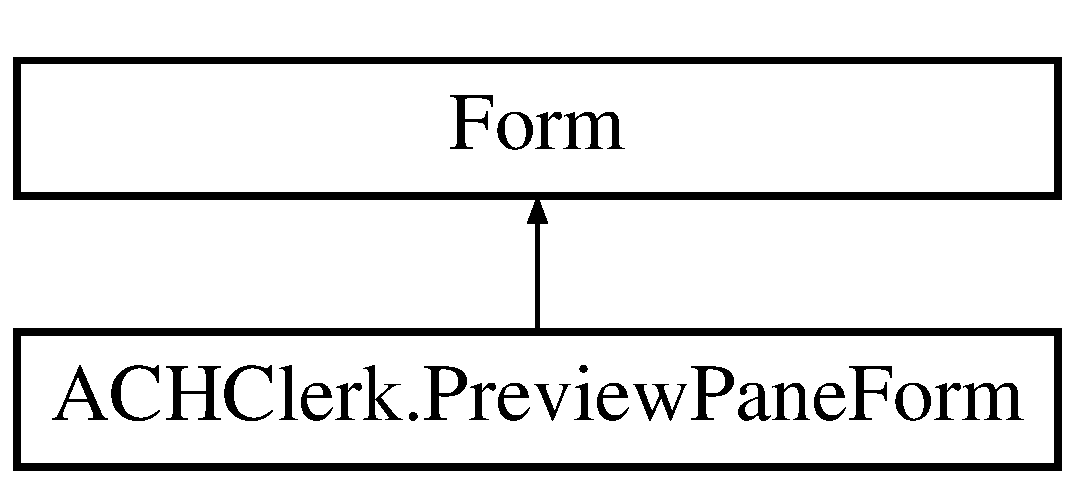
\includegraphics[height=2.000000cm]{class_a_c_h_clerk_1_1_preview_pane_form}
\end{center}
\end{figure}
\subsection*{Public Member Functions}
\begin{DoxyCompactItemize}
\item 
\hyperlink{class_a_c_h_clerk_1_1_preview_pane_form_a550330415c90452efd0750671054066c}{Preview\+Pane\+Form} ()
\begin{DoxyCompactList}\small\item\em Public, default constructor. \end{DoxyCompactList}\item 
\hyperlink{class_a_c_h_clerk_1_1_preview_pane_form_a6ab15c2a4a0f91e09dd758b26e797002}{Preview\+Pane\+Form} (ref Pdf\+Document doc)
\begin{DoxyCompactList}\small\item\em Non-\/default public constructor. Accepts a Pdf\+Document, which will then be used to render a preview of the doc for the user. \end{DoxyCompactList}\end{DoxyCompactItemize}
\subsection*{Protected Member Functions}
\begin{DoxyCompactItemize}
\item 
override void \hyperlink{class_a_c_h_clerk_1_1_preview_pane_form_aae2f2fdd34c0de02247b2682be051af1}{Dispose} (bool disposing)
\begin{DoxyCompactList}\small\item\em Clean up any resources being used. \end{DoxyCompactList}\end{DoxyCompactItemize}


\subsection{Constructor \& Destructor Documentation}
\hypertarget{class_a_c_h_clerk_1_1_preview_pane_form_a550330415c90452efd0750671054066c}{\index{A\+C\+H\+Clerk\+::\+Preview\+Pane\+Form@{A\+C\+H\+Clerk\+::\+Preview\+Pane\+Form}!Preview\+Pane\+Form@{Preview\+Pane\+Form}}
\index{Preview\+Pane\+Form@{Preview\+Pane\+Form}!A\+C\+H\+Clerk\+::\+Preview\+Pane\+Form@{A\+C\+H\+Clerk\+::\+Preview\+Pane\+Form}}
\subsubsection[{Preview\+Pane\+Form}]{\setlength{\rightskip}{0pt plus 5cm}A\+C\+H\+Clerk.\+Preview\+Pane\+Form.\+Preview\+Pane\+Form (
\begin{DoxyParamCaption}
{}
\end{DoxyParamCaption}
)}}\label{class_a_c_h_clerk_1_1_preview_pane_form_a550330415c90452efd0750671054066c}


Public, default constructor. 

\hypertarget{class_a_c_h_clerk_1_1_preview_pane_form_a6ab15c2a4a0f91e09dd758b26e797002}{\index{A\+C\+H\+Clerk\+::\+Preview\+Pane\+Form@{A\+C\+H\+Clerk\+::\+Preview\+Pane\+Form}!Preview\+Pane\+Form@{Preview\+Pane\+Form}}
\index{Preview\+Pane\+Form@{Preview\+Pane\+Form}!A\+C\+H\+Clerk\+::\+Preview\+Pane\+Form@{A\+C\+H\+Clerk\+::\+Preview\+Pane\+Form}}
\subsubsection[{Preview\+Pane\+Form}]{\setlength{\rightskip}{0pt plus 5cm}A\+C\+H\+Clerk.\+Preview\+Pane\+Form.\+Preview\+Pane\+Form (
\begin{DoxyParamCaption}
\item[{ref Pdf\+Document}]{doc}
\end{DoxyParamCaption}
)}}\label{class_a_c_h_clerk_1_1_preview_pane_form_a6ab15c2a4a0f91e09dd758b26e797002}


Non-\/default public constructor. Accepts a Pdf\+Document, which will then be used to render a preview of the doc for the user. 


\begin{DoxyParams}{Parameters}
{\em doc} & \\
\hline
\end{DoxyParams}


\subsection{Member Function Documentation}
\hypertarget{class_a_c_h_clerk_1_1_preview_pane_form_aae2f2fdd34c0de02247b2682be051af1}{\index{A\+C\+H\+Clerk\+::\+Preview\+Pane\+Form@{A\+C\+H\+Clerk\+::\+Preview\+Pane\+Form}!Dispose@{Dispose}}
\index{Dispose@{Dispose}!A\+C\+H\+Clerk\+::\+Preview\+Pane\+Form@{A\+C\+H\+Clerk\+::\+Preview\+Pane\+Form}}
\subsubsection[{Dispose}]{\setlength{\rightskip}{0pt plus 5cm}override void A\+C\+H\+Clerk.\+Preview\+Pane\+Form.\+Dispose (
\begin{DoxyParamCaption}
\item[{bool}]{disposing}
\end{DoxyParamCaption}
)\hspace{0.3cm}{\ttfamily [protected]}}}\label{class_a_c_h_clerk_1_1_preview_pane_form_aae2f2fdd34c0de02247b2682be051af1}


Clean up any resources being used. 


\begin{DoxyParams}{Parameters}
{\em disposing} & true if managed resources should be disposed; otherwise, false.\\
\hline
\end{DoxyParams}


The documentation for this class was generated from the following files\+:\begin{DoxyCompactItemize}
\item 
Preview\+Pane\+Form.\+cs\item 
Preview\+Pane\+Form.\+Designer.\+cs\end{DoxyCompactItemize}

%--- End generated contents ---

% Index
\newpage
\phantomsection
\addcontentsline{toc}{chapter}{Index}
\printindex

\end{document}
